\documentclass[final]{cmpreport}

\usepackage{enumitem}
\usepackage{wasysym}
\usepackage{framed}
\usepackage{pgfgantt,rotating}
\usepackage{subfloat}
\usepackage{listings}
\usepackage{xcolor}
\usepackage{colortbl}

\title{An Evaluation of HTML5\\as a Mobile Gaming Platform}

\author{Joshua Barnett}

\registration{5939968}
\supervisor{Professor Andy Day}

\ccode{CMPC3P2Y}

\summary{
This is my dissertation.
}

\acknowledgements{
These are my achknowledgements
}

\begin{document}

\section{Introduction}
For the past five years it has been evident that mobile devices have risen as one of the foremost dominant ways in which the modern world consumes media and entertainment. Alongside this, a new web standard has been developing. HTML5 (a popularly abused buzzword) is a new language specification with the primary purpose of succeeding where its predecessors failed, in delivering rich interactive content. Generally ``HTML5'' is used as an all encompassing term that includes a host of technologies, as it alone could not deliver such user experiences. Technologies such as JavaScript (JS), Cascasing Style Sheets (CSS), Scalable Vector Graphics (SVG) and WebGL. When used together in varying combinations and configurations these form a Web Platform\footnote{\url{http://docs.webplatform.org/wiki/Main_Page}} on which to convey content and information in new and interesting ways. However, it is currently the convention to refer to this new platform as HTML5.

``Linux'' has similarly been distorted as an all encompassing term for Linux based operating systems such as Debian, Fedora, and Ubuntu. However, ``Linux'' alone is just the open-source kernel which lies at the heart of these distributions but on its own would not be of much use.

OEMs (Original Equipment Manufacturers) such as Apple, LG, Nokia and Samsung are becoming progressively competitive in producing better mobile devices for the global market. They offer higher resolution displays, more memory capacity, and increasingly faster processors. This escalation in performance has been a key instigator in the growing support and optimization of HTML5 and JavaScript on mobiles. However, it has only just begun to reach the requirements needed for delivering interactive real-time graphics applications through HTML5's features, such as video games.

The purpose of this project is to evaluate the current state of the HTML5 and its companion technologies on the mobile platform, and to assess whether they provide a suitable means to develop and deploy games. To assist my research I will be designing and creating my own game, expanding my personal understanding of the platform along the way.

\section{HTML5}
HTML5 is the fifth iteration of the hypertext mark up language. During its previous iterations such as HTML4.01 there was minimal support for multimedia content. This resulted in a void that was promptly filled by third-party plugins such as Adobe Flash and Microsoft Silverlight. Such plugins allowed for easy presentation of media such as video, audio and even allowed for interactivity that was used to great effect in games.

Unfortunately many of these plugins are proprietary and closed-source which prevents developers from fixing and debugging inherent issues in the technology. Instead they are dependant on the technology owner for solutions to these problems while being limited to reporting them or finding ``temporary'' workarounds. Often such plugins also require some form of installation process as they are ``add-ons'' and exist outside of the W3C standard. 

\citet{Jobs} famously professed his concerns about Flash and presented sound reasoning as to why Apple had no intentions of supporting or integrating Flash into their iOS devices. Flash was also briefly available for Android but it was short lived and eventually discontinued by Adobe. Adobe is continuing to making strides into the mobile platform with their new runtime AIR\footnote{\url{https://www.adobe.com/aboutadobe/pressroom/pressreleases/201002/021510FlashPlayerMWC.html}}. HTML5 is still currently a work in progress but the \citet{W3C} have made plans to stabilize the specification and help it reach \textit{Recommendation}\footnote{\url{http://www.w3.org/2005/10/Process-20051014/tr.html\#rec-publication}} status as of this year.

\subsection{The Document Object Model (DOM)}
The document object model (DOM) is the core of what drives modern web applications. It provides a means to manipulate the structure and style of the original document loaded from a web server at run-time on the client side.

However, what makes HTML different from most compiled languages such as C++ and Java, is its a interpreted language. Compiled languages are typically converted into a binary format that compresses their instructions into machine-code allowing for quicker execution. Interpreted languages in contrast are often read line-by-line with their instructions parsed and executed at run-time.

When HTML is interpreted by a web browsers it is parsed into a DOM. The DOM is essentially a representation in memory of what was originally marked down in the static HTML document. This allows the browsers to interpret relations between elements and use them to render the document appropriately. While in memory the information is not longer static allowing for manipulation by other technologies such as JavaScript.

One example of where this manipulation is used to great effect is the single-page application (SPA). SPAs have significant advantages over that of traditional websites as they can provide a seamless user experience similar to that of desktop applications. Instead of navigating through links that loading separate HTML pages they use states to manage the flow, loading information dynamically when required or requested. This methodology shrinks factors such as load times, enables rich interactions, responsiveness while encouraging reuse. \citep{Takada}

\subsection{Web Browsers}
Web browsers are client side applications that render the information requested by the user delivered from a web server. Many of the popular browser vendors such as Google (Chrome), Apple (Safari), and Mozilla (Firefox) all have a mobile counterpart. However these mobile counterparts often support a subset of their desktop editions making much of the fringe HTML5 features even less supported.

\subsection{Cross Compatibility}
Getting a single web application to function and display consistently across a range of browsers can be a huge undertaking. As the specification of HTML5 was being developed much of the features have been implemented in browsers at the discretion of the browser vendor. This has quickly lead to cross compatibility issues as older browsers will support less of these new features and not necessarily be consistent with the other browsers that were also available at the time of release.

One such feature I had planned on using when initially developing my mobile game was \textit{viewport units}. This feature allows for the scaling of elements based upon the viewport's dimensions which is especially useful on mobile devices for scaling visual elements relative to the screen's aspect ratio. However the stock web browsers on mobile devices have almost non-existent support for this feature and has only just started to be introduced in version 4.4 of Android and 6.0 of iOS.

In cases like this a developer can either limit that target platform range and make use of the fringe features available on mobile devices or use a polyfill also known as a shim. A polyfill is often referred to as code that substitutes the lack of a future API by utilising existing features to mimic that of newer fully fledged implementations. \cite{Lawson} I my case I had to polyfill the lack of \textit{viewport units} in older mobile browsers. After searching for a solution I came across the slides of \cite{Kadrmas} presentation that detailed the use of \textit{em} units in HTML5 games. \textit{em} units were originally intended for scaling document elements relative to the current font size. I used this to implement consistent scaling of my game across differing screen sizes by adjusting the root document element's font size relative to the screen width of the current device. This approach also made it easy to retain a specified aspect ratio preventing any oddities when displaying on landscape displays.


\section{Graphics}
When it comes to rendering in HTML5 are I many different options with varying advantages and disadvantages.

\subsection{CSS}
CSS is used to style the way the document elements are rendered. By instructing the browser to use  instructing the browser

\subsection{Canvas}
a

\subsection{SVG}
a

\subsection{WebGL}
WebGL is a distillation of the popular OpenGL making GPU accelerated rendering in the browser now a reality. WebGL, a JavaScript API is based on the OpenGL ES (Embedded Systems) subset, and as the name implies it was designed and optimized for embedded systems such as mobile devices. One streamlined modification OpenGL ES made was the removal of the fixed-function API introduced in OpenGL 1.0 enabling the use and compilation of modern shaders.

WebGL has been in development for the past three years which came to maturity as of early last year when the first a stable version was released. As this is a new technology it has only just begun surfacing in the wild, one notable example is the PlayStation 4's user interface. In a revealing presentation given by Dom Olmstead it was declared that the move to WebGL was done to ensure cross platform support. This potentially hints at Sony's future plans to bring their games to multiple platforms including mobile devices through their PlayStation Now streaming service.

However, the support for WebGL through mobile browsers is essentially nonexistent to date. One company striving to change that is Ludei, who are in the early stages of rolling out their new technology CocoonJS. CocoonJS is a means of packaging and publishing HTML5 applications on mobile devices. In amongst this framework is the facilitation of WebGL letting it tap into the onboard GPU available on most modern mobile devices. Many of the demos they provide demonstrate close to near native performance. This makes WebGL a feasible avenue for game development on mobile devices, with the added bonus of being cross platform ready.

\section{Audio}
a

\subsection{\texttt{<audio>} Element}
a

\subsection{Web Audio API}
a

\subsection{Native Audio}
a

\section{Game Design}
a

\subsection{Player Interaction}
a

\subsection{Gameplay \& Mechanics}
a

\subsection{Feedback}
Throughout the development and prototyping of MindFlip it was important to take into consideration the reactions and feedback of players. So whenever the chance arose I would hand over my phone containing my latest stable build of the game and observe others playing it from a third-party perspective.

Preconceptions can be a double edged sword when used in game design. Often they can be used to draw parallels between activities in contemporary games such as my own. This acts as a shortcut when teaching a player new or similar gameplay mechanics. However, these can also be stumbled upon accidently from a developer's perspective as their own preconceptions about games will likely be vast by comparison to the average player.

This was the case with the initial draft of introductory level. In the beginning the first two card symbols the player encountered were a red nought and a blue cross on a three-by-three grid. After showing the game to my sister while providing no tutorial, the first actions she made were to produce a winning \emph{Tic-tac-toe} game state. This made it apparent that there was a flaw in my game design, because the symbols are common to a pre-existing game namely \emph{Tic-tac-toe} the player receives mixed signals about how to play the game from the offset leading to frustration and confusion. I later decided to go for simpler more abstract symbols such as circles, squares, and triangles in my initial set of levels do to their generic associations they imply simplicity leaving the player open to learn the game mechanics.

\section{Development Stack}
When creating a game targeting HTML5 it can be difficult to know what workflow to invest in. Developers each have their own preferences and beliefs as to what is the best way to work with their priorities often being similar but achieved in different ways.

\subsection{Preprocessors \& Alternatives}
\textit{JavaScript} in its current state (\textit{ECMAScript 5.1}) is an underwhelming language especially when coming from a more mature high-level language background such as \textit{C++} or \textit{Java}. It lacks conventional object-orientated features such as inheritance, generics, and abstraction. The original purpose of \textit{JavaScript} was never intended for the large-scale development it is currently involved in today. And until it's apparent deficiencies are rectified and standardised in its next iteration (\textit{ECMAScript 6}), developers have to over utilise its strengths. To help assist in this transitional period many organisations have been developing alternatives and middle ware to deal with its short comings.

Preprocessors are vastly popular these days amongst developers with their focus often on efficiency. Transpilers (source-to-source compilers) are one such common way in which to improve a developers workflow. With current web languages such as JavaScript and CSS widely supported and heavily standardised by W3C it often takes along time for improvements to make their way into the next specification iteration.
\begin{figure}[h]
  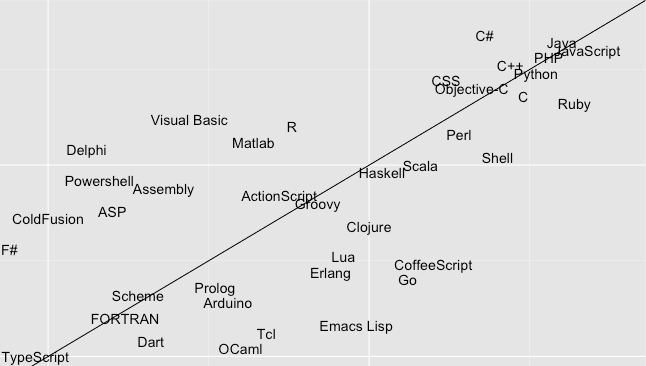
\includegraphics[width=1.0\textwidth]{lang-rank-114-wm.png}
  \caption[The RedMonk Programming Language Rankings: January 2014 (Top 39)]{The RedMonk Programming Language Rankings: January 2014 (Top 39)}
\end{figure}
\footnotetext{\url{http://redmonk.com/sogrady/2014/01/22/language-rankings-1-14/}}
The advantages of transpilers often mean that less can be written in order to achieve the same functionality in its target language. Simple common activities such as writing a for loop to iterate over an array or providing the vendor prefix and polyfills required to support backwards compatibility with older web browsers can be taxing on a developers time. Transpilers can offer an alternative means in which to achieve the same results bit with less code and effort required on the part of the developer.

\subsubsection{Dart}
Google's Dart\footnote{\url{https://www.dartlang.org/}} offers a more uniform pleasant development experience by handling much of the cross-browser compatibility issues behind the scenes. It also contains built-in libraries to handle much of common programming activities; \texttt{``dart:math, dart:json, dart:io, dart:collection...''} as well as familiar functionality similar to jQuery\footnote{\url{http://jquery.com}/} \texttt{``query(), queryAll()''} (one of the most popular JavaScript libraries to date)\footnote{\url{http://trends.builtwith.com/}}, \cite{Fortuna}. Dart compiles down to either machine code that runs on the accompanying DartVM (virtual machine) which is integrated into Google's browser; Chrome, or to an optimized and minified form of JavaScript that'll run in any browser. However there is a significant performance advantage over that of the latter, \cite{Schneider}. 

\subsubsection{TypeScript}
Another alternative to pure JavaScript is Microsoft's TypeScript\footnote{\url{http://www.typescriptlang.org/}} which has taken a more subtle approach. TypeScript is a typed superset of JavaScript that compiles to plain JavaScript which is much more legible when compared with Dart's output making it easier to debug at runtime in-browser. It is still quite a premature project currently in the preview stage but is making significant strides to towards a version 1.0 release, \cite{Turner}. Both approaches have their pros and cons. They are interesting developments and will be intriguing to follow as they evolve along side HTML5.

%\subsubsection{CoffeeScript}
%CoffeeScript\footnote{\url{http://coffeescript.org/}} is a popular alternative to JavaScript with its focus on readability similar to that of other syntactically sugary \cite{Raymond} languages such as Ruby and Python.

%\subsubsection{Sass}
%Sass is a popular CSS preprocessor which addresses many of its shortcomings.

\subsection{JavaScript Modules}
\textit{JavaScript} is typically created as separate \texttt{.js} text files that are then referenced in a \texttt{.html} document by \texttt{<script>} tags. When the web browser finds scripts linked by these tags it will request them from the web server and inject them into the document once loaded. This presents a few problems for large and complex web applications which will often require many scripts each having to be requested and loaded synchronously. Every one of these request has an overhead, which is compounded when a vast quantity are being made. This can lead to suboptimal load times.

To combat this problem a developer could attempt to write all their code in one \texttt{.js} file. This file can quickly become colossal making it difficult to manage and refactor, especially on large scale projects. Alternatively the developer can split their code into several \texttt{.js} files that will all have to be referenced by a corresponding \texttt{<script>} tag. Therefore the more organised the codebase becomes the more requests the browser has to make. The developer also has to micromanage these \texttt{<script>} tags to ensure their ordering is correct. The ordering is important because one script could be referencing another that has not yet been loaded, thus causing runtime errors. This approach also presents issues when attempting to introduce software engineering best practices such as unit testing because the interdependencies between these scripts are not clearly defined.

One solution to this common problem is the \textit{module} design pattern. \textit{JavaScript} has an official name \textit{ECMAScript}, and version \textit{5.1} (ECMA-262\footnote{\url{http://www.ecma-international.org/ecma-262/5.1/}}) is the current standard. However, this present language specification does not support \textit{modules}. The 6th version\footnote{\url{https://people.mozilla.org/~jorendorff/es6-draft.html}} of the \textit{ECMAScript} specification is currently being drafted with plans to include modules but until then developers must seek other alternatives.

There are a variety of libraries that offer solutions such as \textit{RequireJS\footnote{\url{http://requirejs.org/}}}, \textit{HeadJS\footnote{\url{http://headjs.com/}}} and \textit{yepnope.js\footnote{\url{http://yepnopejs.com/}}}. However, personally I found \textit{Browserify\footnote{\url{http://browserify.org/}}} to be the simplest and the most supported amongst the \textit{Node.js} community. \textit{Browserify} enables developers to write their \textit{JavaScript} code in numerous files and when one file requires another it can be injected via the \texttt{require(`example');} function. Once a developer has written all their code they can recursively bundle all their modules starting with a root module similar to that of a main class in conventional programming languages. This provides the developer with the best of both scenarios as all their code will be built into a single \texttt{.js} file (including their external libraries), while allowing for easy management and refactoring of their core codebase through individual source files.

Most might think that this will in turn cause complications when debugging. As when the code breaks it will do so in the colossal \texttt{.js} file that the browser is running. This is where source maps come in. Source maps provide linkage between the original \texttt{.js} source files and their bundled counterparts making breakpoints and stepping through code painless. \cite{Seddon}

This process can also be made seamless by \textit{Watchify} which automatically recompiles the \textit{Browserify} bundle whenever a module file has been updated. This allows for the developer to work on their original source files and as soon as the file has been saved it have rebuilt the bundle ready to reloaded in the browser for testing.

After the modules have been bundled a further step called minification which involves taking legible \textit{JavaScript} and compressing it down into its most minimal form by removing unnecessary characters such as a whitespace and shrinking instance names. This process can further decrease the \texttt{.js} file size making load times marginally faster while also partially obfuscating the original code from prying eyes.

\cite{Hanselman} proclaimed that \textit{JavaScript} has become akin to a assembly language for the web. Which is the impression a lot of people will get when taking a peek at the source of popular website such as \textit{Google} or \textit{Facebook}. This is some what understandable given the that \textit{JavaScript} is as low-level as developers can get when programming for the web. However, a happy side effect of being closely tide with the web is it has become now one of the most portable languages to date, because every web enabled device has a browser, and every browser has a \textit{JavaScript} virtual machine. This makes \textit{JavaScript} a very cross-platform language to develop games with and reaching a wide audience is key when maximising chances for success.

\subsection{Model View Controller (MVC)}
a

\subsection{Templates}
a

\subsection{Build Pipeline}
a

\section{Mobile Deployment}
One of the challenges that faces mobile developers is how to package their applications for the mobile platform, which spans such a wide variety of hardware and operating systems (iOS\footnote{\url{http://www.apple.com/ios/}}, Android\footnote{\url{http://www.android.com/}}, Windows Phone\footnote{\url{http://www.windowsphone.com/}}, Ubuntu\footnote{\url{http://www.ubuntu.com/phone}}), \cite{Feijoo}. This poses a problem especially for the smaller companies as to develop native variants of an application for each platform while retaining a common vision is demanding on both financial and chronological frontiers. Larger companies that facilitate and accommodate such resources, do however frequently benefit from having a superior overall user experience. Most native applications built with their corresponding software development kits have direct access to device specific  application programming intefaces (APIs). This often results in native applications having faster performance and better system user interface integration. Native applications compile to binary machine code that is then interpreted via its relative hardware architecture making it vastly faster than JavaScript which is interpreted at run-time via a browser or web-view. This is most apparent when it comes to developing 3D gaming experiences as these can often be most the most performance taxing, \cite{Kulloli}.

When comparing HTML5 based mobile applications to native there was another significant disadvantage as there was no way to access device APIs. Such APIs are required to make use of the most 

 hardware features on mobile devices such as the camera, device orientation and battery status. Especially considering that each API varies dependant on operating system and then again on hardware specification. For instance not all mobiles have front facing cameras or high-dpi (dots per inch) screens but a vast majority do. So it becomes quite a challenge when trying to build an application that adapts from phone-to-phone without excluding a particular sector of an audience from the core user experience, \cite{Charland}.

A project with the sole purpose of remedying such issues is that of PhoneGap a mobile development framework originally created by a company called Nitboi. After PhoneGap began to make strides the company was purchased and enveloped by Adobe in 2011, \cite{Adobe}. Then after the project matured under Adobe's supervision the project was donated to the Apache Software Foundation. This was to ensure that the project was properly maintained when made open source under the Apache License Version 2.0\footnote{\url{http://www.apache.org/licenses/LICENSE-2.0.html}}. A formality due to this hand over was that the open source variety of the project had to operate under a different name to avoid trademark ambiguity, \cite{Leroux}. Adobe's PhoneGap still functions as a separate entity as a distribution of Apache Cordova offering services such as cloud compilation\footnote{\url{https://build.phonegap.com/}}.

Apache Cordova\footnote{\url{http://cordova.apache.org/}} is a platform for building native mobile applications using HTML, CSS and JavaScript. It achieves this by providing developers with a set of relative device APIs that allow for access of functions previous obfuscated from web technologies by the native system. It also assists with handling a lot of the cross-platform concerns previously mention when targeting multiple platforms and device hardware.

\subsection{Packaging}
a

\subsection{Debugging}
a

\subsection{Profiling}
a


\clearpage
\bibliography{5939968}

\end{document}

